Before we get to the experiments, we will describe the data in this chapter. To get some more insight in to the behaviour of the indexing techniques that we are applying, we perform further analysis of the dat in the hope of getting some useful explanations. We want to ascertain that a typical fingerprint dataset is high dimensional and highly sparse almost follwing a power law sort of distribution with very few features occuring in almost all the points in the chemical database while majority of the features have a non-zero value in very few points. We want to extract patterns in the data which could be exploited for range search querying and point querying.\\

\section{Experiment Datasets}

The two datasets we have explored in this work are from PubChem and DUD. PubChem is a database of chemical compounds and a record of their activities and reactions against agents. It is maintained National Center for Biotechnology Information (NCBI), a component of the National Library of Medicine, which is part of the United States National Institutes of Health (NIH). We have taken a subset of compounds from their database for our experiments. We are using both binary and non-binary fingerprints which have been created using fingerprinting techniques applied on the chemical compound data from their databases. DUD is a directory of useful decoys for benchmarking virtual screening. DUD is provided by the Shoichet Laboratory in the Department of Pharmaceutical Chemistry at the University of California, San Francisco (UCSF). DUD is derived from ZINC, a database of commercially avaiilable compounds. To extarct fingerprints we used MOLPRINT2D, a molecular fingerprinting technique.We will referring to the binary and non-binary versions of the PubChem datasets as PubChem-b and PubChem-n respectively.


\section{A Typical Fingerprint Dataset Analysis}
We perform a detailed analysis of the data from  PubChem -n to figure out the kind of indexing technique, which needs to be used to optimize our searching time. The statistics that were extracted from the data are as follows:\\

\begin{table}[ht!]
\centering
\caption{Statistics of Data}
\begin{tabular}{|l|c|}
\hline 
Number of data points & 264016 \\ 
Number of unique features is & 785985 \\ 
Maximum number of features in a data point is & 1903 \\ 
Minimum number of features in a data point is  & 7 \\ 
Average number of features in a data point is & 270.602966 \\ 
Maximum number of data point with a feature is & 259110 \\ 
Minimum number of data point with a feature is & 1 \\ 
Average number of data point with a feature is & 90
 \\ 
Maximum value of a feature  & 1870 \\ 
Minimum value of a feature
 & 1 \\ 
Average value of a feature & 1.142210 \\ 
Maximum number of heavy-hitters  & 144 \\ 
Minimum number of heavy-hitters  & 1 \\ 
 Average number of heavy-hitters  & 44.5 \\ 
\hline 
\end{tabular} 
\end{table}

From this we can observe that the data is highly sparse with only about 271 features, on a average, in a point, as opposed to the 785985 unique features. This high sparsity makes the data set an ideal candidate to perform inverted indexing. In inverted indexing, instead of indexing the data points we would index the features. This leads to a large index structure, but we gain on the speed of point query. \\

\begin{figure}[ht!]	
\centering
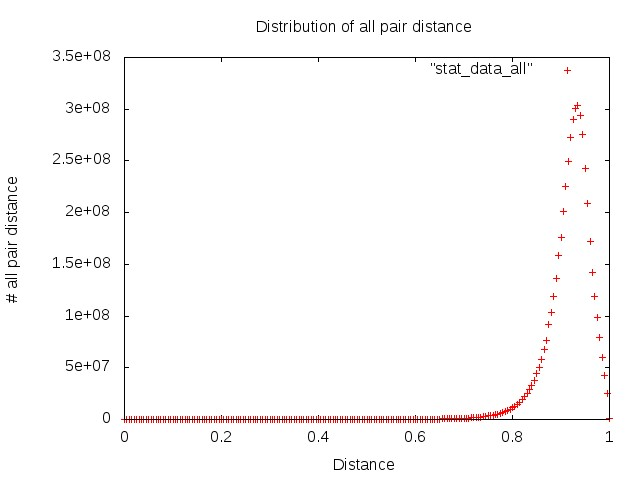
\includegraphics[width=0.7 \columnwidth]{img/all.jpg}
\caption{All pair distances}
\end{figure}
%\pagebreak
\begin{figure}[ht!]	
\centering
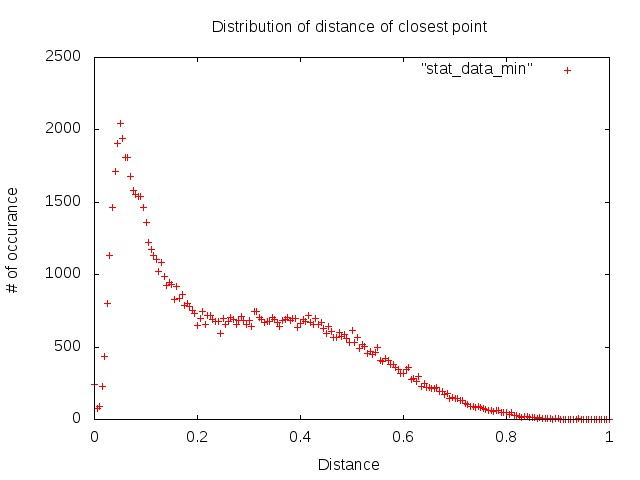
\includegraphics[width=0.7 \columnwidth]{img/min.jpg}
\caption{Distance of the closest point}
\end{figure}

\begin{figure}[ht!]	
\centering
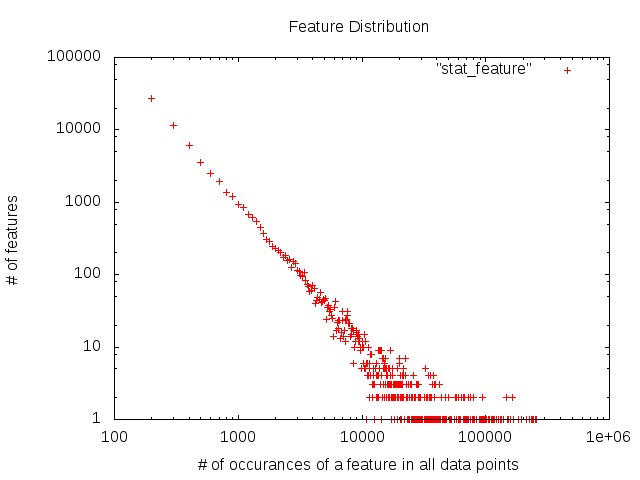
\includegraphics[width=0.7 \columnwidth]{img/feature.jpg}
\caption{Feature distribution}
\end{figure}


\section{Observations on the Data}

We can observe from the data is that them being in high dimension, the points are very much spread out, and hence most of them are equidistant from each other
The closest point for most of the points is at distance much greater than 0.4. in fact only 0.007\% of the points have their 1-NN within a distance of 0.4.

The distribution of features among the data points seem to follow a power law distribution (though we have not tried to regress the plot to a function, this is commonly assumed for chemical data)  i.e., even though we have many features only a hand full of them are repeated in most of the points.

One of the most time consuming operations in our algorithms has been the recurring theme of finding the set of maximally separated points, which we called as pivots. It takes hours for the algorithm to converge. Given the distribution of all pairs distance, we cannot hope to improve it further, but we can propose an heuristic streaming algorithm to handle it efficiently (not explored in this work).

We can maintain a list of most frequently occurring farthest points. These points are not necessarily the points farthest from each other, but the points which are most frequent in the list farthest points, for each point. This is motivated from the frequency counting problem from streaming as shown in \citet*{metwally2005efficient}.

We observed that the baseline inverted index we proposed for point queries could not be easily generalised  to range queries. This can be further observed from the fact that how skewed the data distribution is. Given that only 0.007\% of the 1-nn points have distance less that 0.4, we can never achieve a efficient pruning. And in addition the distribution of heavy-hitters (features with occurrence more that 50000) is also very high, We have on an average 44 heavy hitters in a data point. Hence, in the worst case, we will be forced to explore all the points.

The success of any embedding technique, especially Lipschitz, depends on the ability of the reference set to be representative of the entire data. in our case, given that the entire data is very widely spread, the number of reference set required to well represent the data, becomes very large. This is the reason why Lipschitz did not give the desired results.

